\documentclass{beamer}

\usepackage{cmap}
\usepackage[english,russian]{babel} % add eng,rus(base) package
\usepackage[T1,T2A]{fontenc}        % add eng,rus encoding support
\usepackage[utf8]{inputenc}         % add UTF8 support

% Use it for English document
%\usepackage[utf8]{inputenc} % add UTF8 support
%\usepackage{fontspec}       % to use any font known to the operating system
%\setmainfont{PT Serif}      % set defolt font

\usepackage{amsmath, amsfonts, amssymb, amsthm, mathtools} % add math support

\linespread{1}               % length between str
\setlength{\parindent}{16pt} % red str
\setlength{\parskip}{6pt}   % length between paragraphs

\usepackage[backend=biber, style=authoryear-icomp]{biblatex}
\addbibresource{$HOME/latex-templates/biblio.bib}            % path to bibliography base

\usetheme{Madrid}
\setbeamertemplate{frametitle}[default][center]

\renewcommand{\thefootnote}{\arabic{footnote}}
 % here is document's settings for russian
%\input{$HOME/studyproject/universe/history/preamble-beamer-eng.tex} % here is document's settings for english

\title{Шлем Ярослава Всеволодовича}
\author{Немков Н.М.}
\institute[МГТУ]{МГТУ им. Н.Э. Баумана}
\date{25.09.2023}
\logo{
\includegraphics[width=1cm]{images/logo}}

\begin{document}

\begin{frame}
\maketitle
\end{frame}

\section{Шлем Ярослава Всеволодовича}

\begin{frame}{История шлема}

Будучи смертельно больным, отец передал Ярославу Переяславль-Залесский. В конфликте, возникшем после смерти отца между старшими братьями, Константином и Юрием, Ярослав поддержал Юрия и был разбит вместе с ним в Липицкой битве 1216 года. Во время битвы он потерял свой шлем, который был найден в 1808 году.

\end{frame}
\begin{frame}{Состояние шлема}
	\begin{columns}
		\begin{column}{0.45\textwidth}
			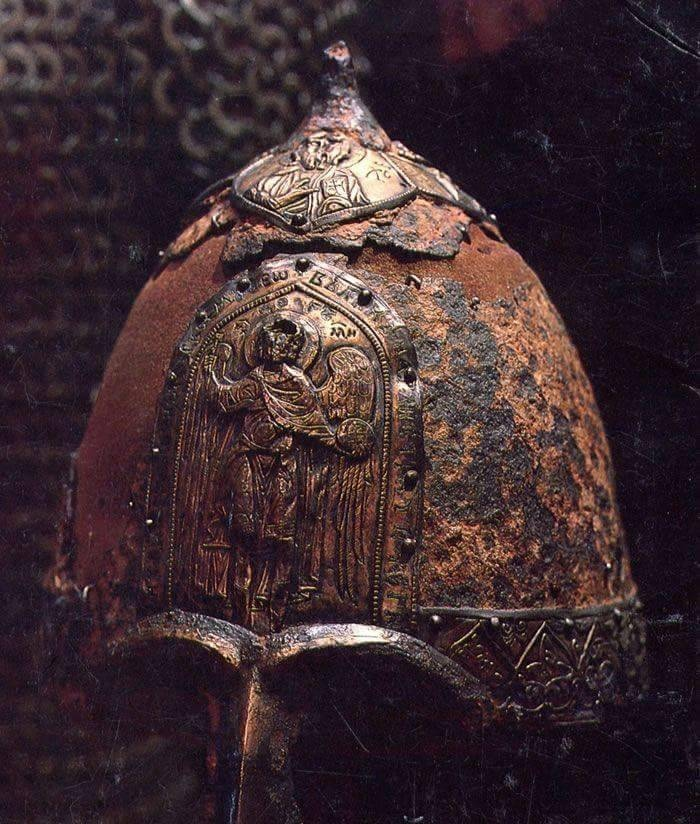
\includegraphics[width=0.9\textwidth]{images/shlem-1.jpg}
		\end{column}
		\begin{column}{0.45\textwidth}

			Тулья\footnote{Основная, верхняя часть головного убора (без полей, околыша, козырька и т.п.).} шлема сохранилась плохо — в виде двух крупных частей, поэтому нельзя точно определить её форму и конструкцию.

			Корпус шлема покрыт серебряным листом, украшен позолоченными серебряными чеканными накладками.

		\end{column}
	\end{columns}
\end{frame}
\begin{frame}{Состояние шлема}

	Наверху — образа Вседержителя, святых Георгия, Василия и Феодора. На налобной пластине — образ Архангела Михаила и черневая надпись: «Вьликъи архистратиже ги Михаиле помози рабу свуему Феодору»\footnote{Великий Архангел Михаил, помоги слуге Твоему Феодору}. По краю шлема — орнаментальная кайма.

\end{frame}
\begin{frame}{Состояние шлема}
	\begin{columns}
		\begin{column}{0.45\textwidth}

	По данным Бориса Колчина, тулья шлема является цельнокованной и изготовлена из железа или малоуглеродистой стали техникой штамповки с последующей выколоткой, что отличает его от других шлемов данного типа, равно как и других типов данного периода. При изготовлении шлема она была предварительно набита серебряным листом.

		\end{column}
		\begin{column}{0.45\textwidth}

			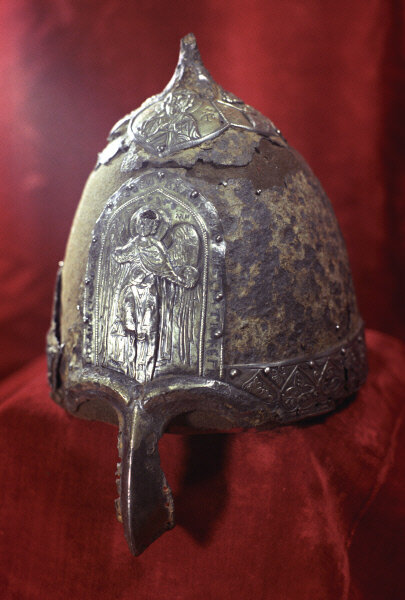
\includegraphics[width=0.9\textwidth]{images/shlem-2.jpg}

		\end{column}
	\end{columns}
\end{frame}
\begin{frame}{Состояние шлема}
	\begin{columns}
		\begin{column}{0.45\textwidth}
			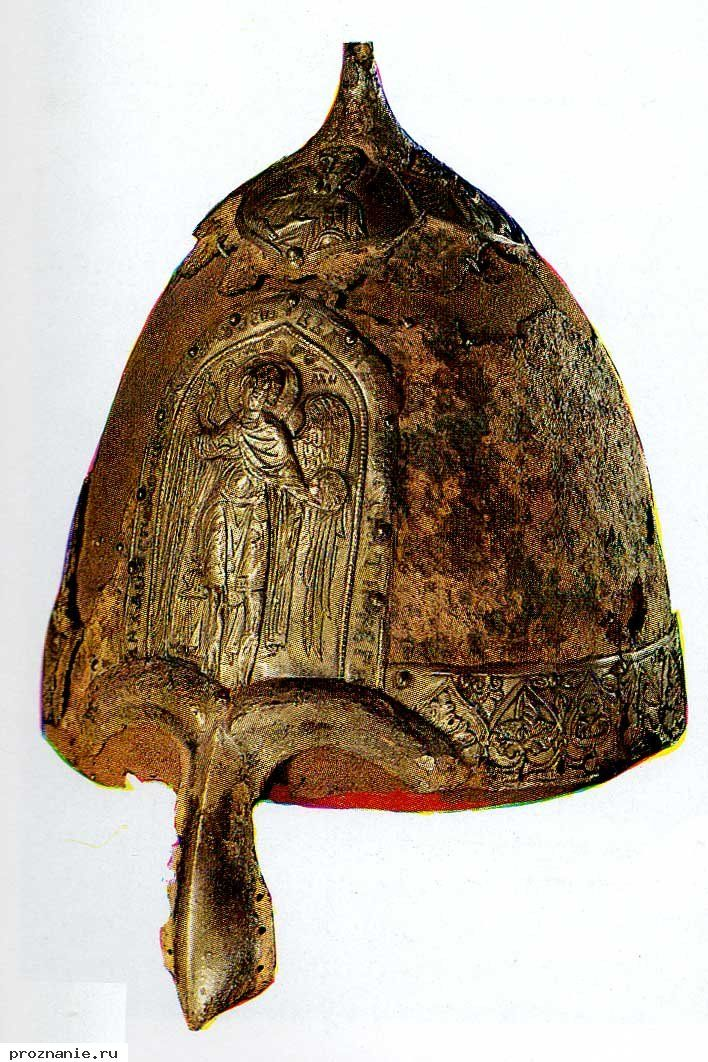
\includegraphics[width=0.9\textwidth]{images/shlem-3.jpg}
		\end{column}
		\begin{column}{0.45\textwidth}

			К 2021 году шлем был впервые отреставрирован реставратором музеев Московского Кремля Михаилом Кружалиным.

		\end{column}
	\end{columns}
\end{frame}

\section{References}

\begin{frame}[t]{References}
	\printbibliography
	\url{https://dic.academic.ru/dic.nsf/ushakov/1060158}
	\url{https://stuki-druki.com/authors/Yaroslav-Wsevolodovich.php}
\end{frame}

\section{Благоданость}
\begin{frame}
	\centering
	\huge
	Спасибо за внимание!
\end{frame}

\end{document}
